% ============================================================================
% REQUIRED PACKAGES & CONFIGURATIONS FOR COMPILING THIS EXPERIMENT:
% ----------------------------------------------------------------------------
% \usepackage{circuitikz}      % For drawing electrical circuit diagrams
% \usepackage{pgfplots}        % For professional scientific plotting
% \pgfplotsset{compat=1.18}    % Ensures modern rendering engine defaults
% \usepackage{booktabs}        % For high-quality, publication-grade tables
% \usepackage{amsmath}         % For advanced mathematical typesetting
% \usepackage{siunitx}         % For standard units (\SI, \kilo\omega, etc.)
% ============================================================================

\chapter{MOSFET Amplifier in CS Configuration -- Measurement of Gain, Bandwidth, and Plotting of Frequency Response}

\section{Aim}
To design, set up, and test a single-stage Common Source (CS) MOSFET amplifier using a voltage-divider bias configuration. The specific objectives are:
\begin{enumerate}
	\item To determine and verify the DC operating point ($Q$-point) of the MOSFET.
	\item To measure the mid-band voltage gain of the CS amplifier.
	\item To plot the frequency response curve (Gain in dB vs Frequency) on a semi-logarithmic scale.
	\item To evaluate the lower cutoff frequency ($f_L$), upper cutoff frequency ($f_H$), and overall bandwidth ($BW$).
\end{enumerate}

\section{Pre-Lab Assignment}
Before performing the experiment, students must complete the following analytical tasks:
\begin{enumerate}
	\item For the circuit specified in the Design section ($V_{DD} = \SI{12}{\volt}$, $R_1 = \SI{1}{\mega\Omega}$, $R_2 = \SI{470}{\kilo\Omega}$, $R_D = \SI{2.2}{\kilo\Omega}$, $R_S = \SI{560}{\Omega}$), calculate the theoretical DC operating point parameters ($V_G$, $V_S$, $I_D$, and $V_{DS}$). Assume the N-channel MOSFET has a threshold voltage $V_{GS(th)} = \SI{2.0}{\volt}$ and conduction parameter $K_n = \SI{2.0}{\milli\ampere\per\volt\squared}$.
	\item Sketch the small-signal equivalent AC circuit of the Common Source amplifier and derive the expression for the mid-band voltage gain ($A_v$).
	\item Compare a MOSFET Common Source amplifier with a BJT Common Emitter amplifier in terms of input impedance, output impedance, and voltage gain.
	\item Explain why the source bypass capacitor ($C_S$) is necessary and how its removal would impact the amplifier's input impedance and voltage gain.
\end{enumerate}

\section{Components and Equipment Required}
The components and test instruments required for this experiment are listed in Table \ref{tab:components_mosfet}.

\begin{table}[h!]
	\centering
	\caption{Components and Equipment Specifications}
	\label{tab:components_mosfet}
	\begin{tabular}{llll}
		\toprule
		\textbf{S. No.} & \textbf{Item Name} & \textbf{Specification / Range} & \textbf{Quantity} \\
		\midrule
		1 & MOSFET & N-Channel Enhancement (2N7000 or BS170) & 1 No. \\
		2 & Resistors & \SI{1}{\mega\Omega}, \SI{470}{\kilo\Omega}, \SI{2.2}{\kilo\Omega}, \SI{560}{\Omega}, \SI{10}{\kilo\Omega} (Load) & 1 No. each \\
		3 & Capacitors & \SI{1}{\micro\farad} (Electrolytic), \SI{47}{\micro\farad} (Electrolytic) & 2 Nos., 1 No. \\
		4 & Dual Regulated Power Supply & $0 - 30\text{ V}$, $1\text{ A}$ (DC) & 1 No. \\
		5 & Function Generator & $1\text{ Hz} - 1\text{ MHz}$, Sinusoidal output & 1 No. \\
		6 & Digital Storage Oscilloscope (DSO) & Dual channel, \SI{20}{\mega\hertz} or higher & 1 No. \\
		7 & Breadboard \& Connecting Wires & Standard multi-contact, single-strand wires & As required \\
		\bottomrule
	\end{tabular}
\end{table}

\section{Theory}
The Common Source (CS) configuration of a Metal-Oxide-Semiconductor Field-Effect Transistor (MOSFET) is highly valued in analog electronics primarily due to its exceptionally high input impedance, which approaches infinity at DC and low frequencies. This characteristic prevents the amplifier stage from loading down the preceding signal source.

\subsection{Circuit Functionality}
\begin{itemize}
	\item \textbf{Voltage-Divider Biasing ($R_1, R_2$):} Since the insulated gate of a MOSFET draws virtually zero DC current ($I_G \approx 0$), the gate voltage $V_G$ is established purely by the voltage divider network across the supply rail $V_{DD}$. This arrangement provides an exceptionally stable operating point.
	\item \textbf{Drain and Source Resistors ($R_D, R_S$):} $R_D$ dictates the quiescent drain voltage and converts the dynamic AC drain current into an amplified voltage signal. $R_S$ provides self-bias stabilization against device parameter variations.
	\item \textbf{Coupling and Bypass Capacitors ($C_{in}, C_{out}, C_S$):} $C_{in}$ and $C_{out}$ isolate the DC bias voltages of the stage from the input source and output load. The source bypass capacitor $C_S$ provides an AC short circuit across $R_S$ to ground, preventing negative feedback (degeneration) from reducing the mid-band AC voltage gain.
\end{itemize}

\subsection{Frequency Response Characteristics}
Similar to other RC-coupled architectures, the voltage gain drops off at extreme frequencies:
\begin{enumerate}
	\item \textbf{Low-Frequency Roll-off:} Dominated by the increasing series reactances of $C_{in}$ and $C_{out}$, along with the parallel impedance of $C_S$. As the frequency approaches DC, these components attenuate the signal or introduce internal degeneration.
	\item \textbf{Mid-Band Plateau:} The coupling/bypass capacitors act as optimal short circuits while internal parasitic capacitances remain open. The voltage gain remains flat at its maximum value, given by:
	\begin{equation}
		A_{v(mid)} \approx -g_m (R_D \parallel R_L)
	\end{equation}
	where $g_m$ represents the transconductance of the MOSFET at its given operating point.
	\item \textbf{High-Frequency Roll-off:} Caused by internal device capacitances (gate-to-source $C_{gs}$, gate-to-drain $C_{gd}$) and stray wiring capacitance. The effective input capacitance is heavily multiplied due to the Miller effect, shunting high-frequency signals to ground.
\end{enumerate}

The system bandwidth is evaluated using the upper ($f_H$) and lower ($f_L$) frequencies where the gain falls by \SI{3}{\decibel} ($70.7\%$) from its mid-band value:
\begin{equation}
	BW = f_H - f_L
\end{equation}

\section{Circuit Diagram}
The schematic for the single-stage voltage-divider biased CS MOSFET amplifier is presented in Figure \ref{fig:mosfet_circuit}.

\begin{figure}[h!]
	\centering
	\begin{circuitikz}[scale=1.2, line width = 0.85pt, transform shape]
		% MOSFET node
		\draw (3,2) node[nmos] (m1) {2N7000};
		
		% Input source and capacitor
		\draw (-1.5,2) to[sV, l_=$v_s(t)$] (-1.5,0) node[ground] {};
		\draw (-1.5,2) to[C, l=$C_{in}$] (0.5,2);
		\draw (0.5,2) -- (m1.G);
		
		% Biasing Resistors
		\draw (0.5,2) to[R, l=$R_1$] (0.5,4.5);
		\draw (0.5,2) to[R, l_=$R_2$] (0.5,0) node[ground] {};
		
		% Drain circuit
		\draw (m1.D) to[R, l_=$R_D$] (3,4.5);
		\draw (m1.D) -- (5,2.75) to[C, l=$C_{out}$] (6.5,2.75);
		
		% Source circuit
		\draw (m1.S) to[R, l_=$R_S$] (3,0) node[ground] {};
		\draw (3, 1.4) -- (4.2,1.4) to[C, l=$C_S$] (4.2,0) node[ground] {};
		
		% Supply rail
		\draw (0.5,4.5) -- (3,4.5) -- (5,4.5) node[right] {$V_{DD} = +12\text{ V}$};
		
		% Output load
		\draw (6.5,2.75) to[R, l=$R_L$] (6.5,0) node[ground] {};
		\draw (6.5,2.75) -- (7.5,2.75) node[right] {$V_{out}$};
		
		% Connection dots
		\node[circle, fill, inner sep=1.5pt] at (0.5,2) {};
		\node[circle, fill, inner sep=1.5pt] at (3,4.5) {};
		\node[circle, fill, inner sep=1.5pt] at (0.5,4.5) {};
		\node[circle, fill, inner sep=1.5pt] at (3,1.4) {};
		\node[circle, fill, inner sep=1.5pt] at (6.5,2.75) {};
		\node[circle, fill, inner sep=1.5pt] at (m1.D) {};
	\end{circuitikz}
	\caption{Circuit Diagram of a Single-Stage Voltage-Divider Biased CS MOSFET Amplifier}
	\label{fig:mosfet_circuit}
\end{figure}

\section{Design}
\subsection{Design Specifications}
Let us design the amplifier for the following typical experimental parameters:
\begin{itemize}
	\item Supply Voltage, $V_{DD} = \SI{12}{\volt}$
	\item Quiescent Drain Current, $I_D = \SI{2}{\milli\ampere}$
	\item MOSFET Conduction Parameter, $K_n = \SI{2}{\milli\ampere\per\volt\squared}$
	\item MOSFET Threshold Voltage, $V_{GS(th)} = \SI{2.0}{\volt}$
\end{itemize}

\subsection{Step-by-Step Design Procedure}
\begin{enumerate}
	\item \textbf{Design of $R_S$:} To safeguard against thermal runaway and track variations smoothly, allocate roughly $10\%$ of $V_{DD}$ across the source resistor $R_S$:
	\begin{equation}
		V_S = 0.1 \times V_{DD} = 0.1 \times 12\text{ V} = \SI{1.2}{\volt}
	\end{equation}
	Given $I_D = \SI{2}{\milli\ampere}$:
	\begin{equation}
		R_S = \frac{V_S}{I_D} = \frac{1.2\text{ V}}{2\text{ mA}} = \SI{600}{\Omega} \quad (\text{Select standard value: } \SI{560}{\Omega})
	\end{equation}
	
	\item \textbf{Design of $R_D$:} For balanced signal swing, aim to drop approximately half of the remaining supply headroom across the drain resistor $R_D$:
	\begin{equation}
		V_{RD} = \frac{V_{DD} - V_S}{2} = \frac{12\text{ V} - 1.2\text{ V}}{2} = \SI{5.4}{\volt}
	\end{equation}
	\begin{equation}
		R_D = \frac{V_{RD}}{I_D} = \frac{5.4\text{ V}}{2\text{ mA}} = \SI{2.7}{\kilo\Omega} \quad (\text{Select standard value: } \SI{2.2}{\kilo\Omega} \text{ for robust bias padding})
	\end{equation}
	
	\item \textbf{Design of Biasing Network ($R_1$ and $R_2$):}
	Using the saturation region current equation to find the operational $V_{GS}$:
	\begin{equation}
		I_D = K_n (V_{GS} - V_{GS(th)})^2 \implies 2\text{ mA} = 2\text{ mA/V}^2 \cdot (V_{GS} - 2\text{ V})^2
	\end{equation}
	\begin{equation}
		(V_{GS} - 2\text{ V}) = 1 \implies V_{GS} = \SI{3.0}{\volt}
	\end{equation}
	Consequently, the required absolute gate voltage $V_G$ relative to ground is:
	\begin{equation}
		V_G = V_{GS} + V_S = 3.0\text{ V} + 1.2\text{ V} = \SI{4.2}{\volt}
	\end{equation}
	Since $I_G = 0$, select very large mega-ohm scale values for $R_1$ and $R_2$ to uphold high input resistance. Setting $R_1 = \SI{1}{\mega\Omega}$:
	\begin{equation}
		V_G = V_{DD} \left( \frac{R_2}{R_1 + R_2} \right) \implies 4.2 = 12 \left( \frac{R_2}{1\text{ M}\Omega + R_2} \right) \implies R_2 \approx \SI{538}{\kilo\Omega}
	\end{equation}
	Choose standard laboratory values: $R_1 = \SI{1}{\mega\Omega}$ and $R_2 = \SI{470}{\kilo\Omega}$.
\end{enumerate}

\section{Procedure}
\subsection{DC Operating Point Verification (Static Analysis)}
\begin{enumerate}
	\item Set up the discrete components on the breadboard based on the schematic in Figure \ref{fig:mosfet_circuit}. Keep the signal source and the load resistor disconnected at this step.
	\item Power up the bench supply, setting $V_{DD} = \SI{12}{\volt}$.
	\item Use a digital multimeter to record the static voltages at the Gate ($V_G$), Source ($V_S$), and Drain ($V_D$) nodes relative to ground.
	\item Compute the operational quiescent parameters: $V_{GS} = V_G - V_S$, $V_{DS} = V_D - V_S$, and $I_D = V_S / R_S$. Record these in Table \ref{tab:dc_obs_mos} and check if the device is correctly biased in its saturation region ($V_{DS} \ge V_{GS} - V_{GS(th)}$).
\end{enumerate}

\subsection{AC Analysis and Frequency Response Plotting}
\begin{enumerate}
	\item Couple the input signal generator to $C_{in}$. Hook up DSO Channel 1 at the input node to keep track of $V_{in}$ and Channel 2 across the terminal load resistor $R_L$ to register $V_{out}$.
	\item Program the generator to yield a standard sinusoidal trace at an initial benchmark mid-band frequency of \SI{1}{\kilo\hertz}.
	\item Attenuate the input amplitude ($V_{in}$) to a modest level (e.g., $50\text{ mV}_{p-p}$). Monitor Channel 2 to ensure the output waveform is highly symmetric and free from clipping or cross-over distortion.
	\item Carefully lock and maintain this input voltage level $V_{in}$ constant throughout the remaining frequency sweep steps.
	\item Step the frequency progressively from \SI{10}{\hertz} out to \SI{1}{\mega\hertz} using uniform logarithmic increments.
	\item Log the peak-to-peak voltage value for $V_{out}$ in Table \ref{tab:ac_obs_mos} at each specified frequency tier.
	\item Evaluate the numeric voltage gain $A_v = V_{out} / V_{in}$ and compute the proportional decibel scaling: $A_v \text{ (dB)} = 20\log_{10}(A_v)$.
	\item Graph the logged results using a semi-logarithmic grid, assigning Gain (dB) to the linear y-axis and Frequency (Hz) to the logarithmic x-axis.
	\item Locate the peak plateau ($A_{v(mid)}$). Drop a horizontal coordinate line exactly \SI{3}{\decibel} below this ceiling. The intersection points will resolve the lower cutoff frequency ($f_L$) and upper cutoff frequency ($f_H$). Find the total bandwidth using $BW = f_H - f_L$.
\end{enumerate}

\section{Precautions}
\begin{enumerate}
	\item \textbf{Electrostatic Discharge (ESD) Awareness:} MOSFETs possess extremely thin insulated gate oxide barriers that are highly vulnerable to static electricity. Ground your hands before handling the transistor pins and do not insert or remove components while the power supply is turned on.
	\item \textbf{Signal Compression Constraints:} Ensure $V_{in}$ does not drive the output near the saturation or cutoff boundaries. If the output peaks begin to flatten, immediately scale down the signal generator's output level.
	\item \textbf{Bypass Capacitor Integrity:} Double-check that the electrolytic capacitors are oriented correctly with respect to node potentials to avoid leakage currents destabilizing the operating point.
\end{enumerate}

\section{Model Graph / Expected Waveforms}
The typical performance characteristic curve for the configured CS amplifier is presented in Figure \ref{fig:model_graph_mos}.

\begin{figure}[h!]
	\centering
	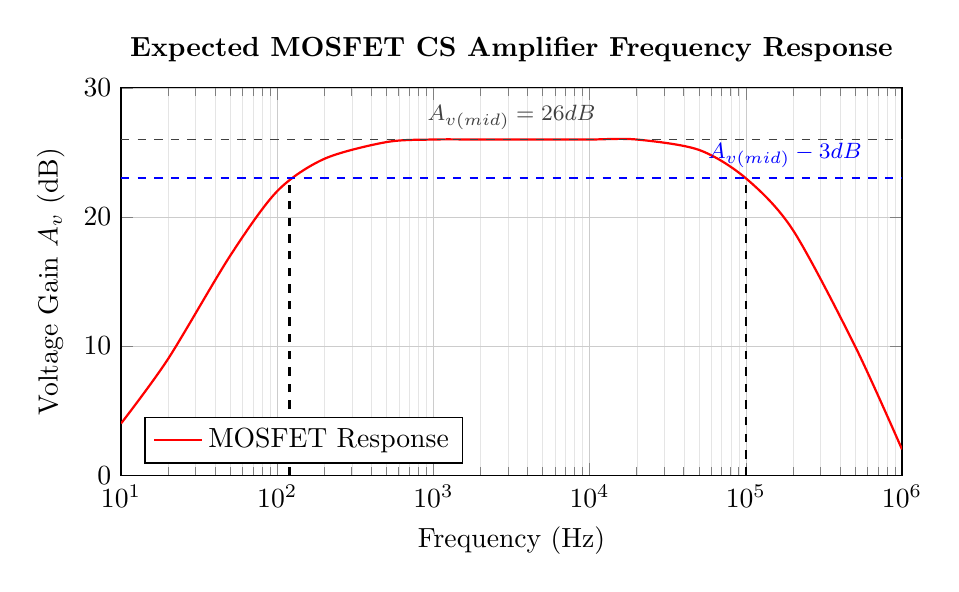
\begin{tikzpicture}
		\begin{semilogxaxis}[
			xlabel={Frequency (Hz)},
			ylabel={Voltage Gain $A_v$ (dB)},
			xmin=10, xmax=1000000,
			ymin=0, ymax=30,
			grid=both,
			grid style={line width=.1pt, draw=gray!20},
			major grid style={line width=.2pt, draw=gray!40},
			width=11.5cm, height=6.5cm,
			title={\textbf{Expected MOSFET CS Amplifier Frequency Response}},
			legend pos=south west
			]
			% Simulated smooth gain data for MOSFET
			\addplot[thick, color=red, smooth] coordinates {
				(10, 4) (20, 9) (50, 17) (100, 22) (200, 24.5) (500, 25.8)
				(1000, 26) (2000, 26) (5000, 26) (10000, 26) (20000, 26)
				(50000, 25.2) (100000, 23) (200000, 19) (500000, 10) (1000000, 2)
			};
			\addlegendentry{MOSFET Response}
			
			% Midband level and -3dB line
			\draw[dashed, blue, thick] (axis cs:10, 23) -- (axis cs:1000000, 23) node[above, pos=0.85] {\footnotesize $A_{v(mid)} - 3\text{ dB}$};
			\draw[dashed, darkgray, thin] (axis cs:10, 26) -- (axis cs:1000000, 26) node[above, pos=0.5] {\footnotesize $A_{v(mid)} = 26\text{ dB}$};
			
			% Cutoff markers
			\draw[dashed, black, thick] (axis cs:120, 0) -- (axis cs:120, 23);
			\draw[dashed, black, thick] (axis cs:100000, 0) -- (axis cs:100000, 23);
			
			% Labels for cutoff points
			\node[below] at (axis cs:120, 0) {$f_L$};
			\node[below] at (axis cs:100000, 0) {$f_H$};
		\end{semilogxaxis}
	\end{tikzpicture}
	\caption{Semi-logarithmic plot of the Expected Frequency Response}
	\label{fig:model_graph_mos}
\end{figure}

\section{Observation Tables}
\subsection{DC Operating Point Parameters}
Compare the static baseline target parameters against actual laboratory multimeter readings in Table \ref{tab:dc_obs_mos}.

\begin{table}[h!]
	\centering
	\caption{DC Biasing Values}
	\label{tab:dc_obs_mos}
	\begin{tabular}{llll}
		\toprule
		\textbf{Parameter} & \textbf{Theoretical Value} & \textbf{Practical Value (Measured)} & \textbf{\% Deviation} \\
		\midrule
		Gate Voltage ($V_G$) & \SI{3.83}{\volt} & & \\
		Source Voltage ($V_S$) & \SI{1.12}{\volt} & & \\
		Drain Voltage ($V_D$) & \SI{7.60}{\volt} & & \\
		Gate-Source Voltage ($V_{GS}$) & \SI{2.71}{\volt} & & \\
		Drain-Source Voltage ($V_{DS}$) & \SI{6.48}{\volt} & & \\
		Drain Current ($I_D$) & \SI{2.0}{\milli\ampere} & & \\
		\bottomrule
	\end{tabular}
\end{table}

\subsection{AC Frequency Response Data}
Log the raw output amplitudes across the sweep spectrum in Table \ref{tab:ac_obs_mos}, ensuring $V_{in}$ remains fixed.

\begin{table}[h!]
	\centering
	\caption{AC Frequency Sweep Measurements}
	\label{tab:ac_obs_mos}
	\begin{tabular}{cccccc}
		\toprule
		\textbf{S. No.} & \textbf{Frequency (Hz)} & \textbf{Input $V_{in}$ (V)} & \textbf{Output $V_{out}$ (V)} & \textbf{Gain $A_v = \frac{V_{out}}{V_{in}}$} & \textbf{Gain in dB $= 20\log_{10}(A_v)$} \\
		\midrule
		1 & 10 & & & & \\
		2 & 20 & & & & \\
		3 & 50 & & & & \\
		4 & 100 & & & & \\
		5 & 200 & & & & \\
		6 & 500 & & & & \\
		7 & 1k & & & & \\
		8 & 2k & & & & \\
		9 & 5k & & & & \\
		10 & 10k & & & & \\
		11 & 20k & & & & \\
		12 & 50k & & & & \\
		13 & 100k & & & & \\
		14 & 200k & & & & \\
		15 & 500k & & & & \\
		16 & 1M & & & & \\
		\bottomrule
	\end{tabular}
\end{table}

\section{Result}
The specific performance metrics of the voltage-divider biased single-stage Common Source MOSFET amplifier were successfully mapped and derived:
\begin{itemize}
	\item Maximum Mid-Band Voltage Gain, $A_{v(mid)}$ = \rule{2cm}{0.15mm} (or \rule{2cm}{0.15mm} dB)
	\item Lower Cutoff Frequency, $f_L$ = \rule{2cm}{0.15mm} Hz
	\item Upper Cutoff Frequency, $f_H$ = \rule{2cm}{0.15mm} Hz
	\item Measured Amplifier Bandwidth ($BW = f_H - f_L$) = \rule{2cm}{0.15mm} Hz
\end{itemize}
The baseline $Q$-point parameters were verified to support operation within the saturation region, and the frequency response confirms high-frequency roll-off due to parasitic device effects.

\section{Questions}
\begin{enumerate}
	\item Why does the input impedance of a MOSFET amplifier drop when operating at very high frequencies?
	\item What is meant by the term "Transconductance" ($g_m$) of a MOSFET, and how does it affect the voltage gain?
	\item Explain the criteria required to ensure an enhancement-mode N-channel MOSFET remains in its saturation region for large signal swings.
	\item How does adding a load resistor ($R_L$) in parallel with the output alter the upper and lower cutoff frequencies?
	\item What is the significance of the Miller effect, and which parasitic internal capacitance is responsible for dragging down the high-frequency response in a CS amplifier?
\end{enumerate}